\section{Assignment 1}
The goal of this assignment is to find the equilibria of a energy balance equation based on a very simplified model of the Earth.
Additionally, we perform a one parameter analysis using continuation on a parameter that represents the greenhouse effect. 
This allows us to study the bifurcation diagram of the model.

% table of variables and their meanings
\begin{table}[H]
    \centering
    \begin{tabular}{|c|c|c|c|}
        \hline
        Variable & Unit &  Meaning & Value\\
        \hline
        $\theta$ & - & latitude & $[-\frac{\pi}{2}, \frac{\pi}{2}]$\\
        $t $ & $s$ & time & -\\
        $x = \sin \theta$ & -  & latitude coordinate & $[-1, 1]$\\
        $T $ & $K$ & temperature & -\\
        $R_A $ & $J s^{-1} m^{-2}$ & effective solar radiation & - \\
        $Q $ & $J s^{-1} m^{-2}$ & solar radiation & -\\
        $Q_0 $ & $J s^{-1} m^{-2}$ & solar radiation constant & 341.3\\
        $\alpha$ & - & albedo of Earth & -\\
        $\alpha_1$ & - & albedo of ice & 0.7\\
        $\alpha_2$ & - & albedo of water & 0.289\\
        $T^{*} $ & K & temperature at which ice melts & 273.15\\
        $M$ & $K^{-1}$ & temperature gradient (?) & -\\
        $\mu $ & $J s^{-1} m^{-2}$ & greenhouse gas \& fine particle parameter & 30\\
        $R_E $ & $J s^{-1} m^{-2}$ & black body radiation & -\\
        $h_0$ & - & emmisivity of Earth & 0.61\\
        $\sigma_0 $ & $J s^{-1} m^{-2} K^{-4}$ & Stefan-Boltzmann constant & $5.67 \cdot 10^{-8}$\\
        $R_D $ & $J s^{-1} m^{-2}$ & heat dispersion & -\\
        $D $ & $J s^{-1} m^{-2}$ & heat dispersion constant & 0.3\\
        $\delta $ & $J s^{-1} m^{-2}$ & heat dispersion at poles & 0\\
        $C_T $ & $J K^{-1}$  & heat capacity of Earth & $5 \cdot 10^{8}$\\
        \hline
    \end{tabular}
    \caption{Variables and their meanings}
    \label{tab:vars}
\end{table}

\subsection{Boundary Conditions}
    $\delta$ cannot be positive (resp. negative) at $x = \pm 1$ (poles), otherwise energy would be
    artificially entering (resp. leaving) the system. Simply said, the poles cannot be a source or sink of energy.
    This requires us to set $\delta = 0$ at $x = \pm 1$. Furthemore 
    \begin{align*}
            \left.\frac{d T}{dx}\right|_{x = \pm 1} = 0.
    \label{eq:bcs}
    \end{align*}
    However, we run into a problem when we combine the boundary conditions and set $\delta = 0$. The 
    equation for the heat dispersion vanishes at the boundary and we are left with two algebraic equations in terms 
    of $T(\pm 1)$
    \begin{align*}
        \left.R_A(T, x) - R_E(T)\right|_{x=\pm1} = 0.  
    \end{align*} 
    Solving these equations for $T(\pm 1)$ gives us the equilibrium temperature at the poles
    \begin{align*}
        T_eq(\pm 1) \approx 220.5 K,
    \end{align*}
    for the values speciefied in table \ref{tab:vars}.
    
    Alternatively, we can resort to a more basic requirement. Namely, that there must exist an equilibrium temperature $T_0$ at the poles,
    \begin{align*}
        &\left.F(T(x, t))\right|_{x=\pm 1} = 0, \quad \forall t > 0,\\
        &\implies \left.-2x\frac{dT}{dx} + R_A - R_E\right|_{x=\pm 1} = 0.
    \end{align*}
    Assuming we use the given expansion of T in terms of legendre polynomials, we can write the above as
    \begin{align*}
        \sum_{n=0}^{\infty} \left. 2x\frac{\lambda_n}{D} a_n\frac{d \phi_n}{dt} -(R_A - R_E) \right|_{x=\pm 1}= 0,\\
        \implies
        \begin{cases}
            \sum_{n=0}^{\infty} \frac{\lambda_n^2 a_n}{D} = \left. R_A - R_E \right|_{x=1},\\
            \sum_{n=0}^{\infty} (-1)^n\frac{\lambda_n^2 a_n}{D} = \left. -R_A + R_E \right|_{x=-1},\\
        \end{cases},
    \end{align*}
    where we used the properties 
    \begin{align*}
        \frac{d\phi_n(1)}{dx} = \frac{\lambda_n}{2} \quad \textrm{and} \quad \phi_n(-x) = (-1)^n \phi_n(x).
    \end{align*}

\subsection{Discretisation}
We choose to decompose the temperature field into a sum of orthogonal Legendre polynomials, i.e.
\begin{align*}
    T(x) = \sum_{n=0}^{\infty} a_n \phi_n(x),
\end{align*}
where the timedependence is dropped seeing as we are after equilibrium solutions.

Subsitution of the above in the (equilibrium) energy balance equation yields
\begin{align*}
    -\sum_{i=0}^{\infty} \frac{\lambda_n a_n}{D} \phi_n + R_A(T,x) + R_E(T) = 0.
\end{align*}
We now use Galerkin's method to project the above equation onto the Legendre basis functions. This gives
\begin{align*}
    F_i(T(\mathbf{a})) = \int_{-1}^{1} \left[-\sum_{i=0}^{\infty} \frac{\lambda_n a_n}{D}\phi_n + R_A(T,x) + R_E(T)\right] \phi_i dx = 0.
\end{align*}
where $F_i$ is the ith component of discretised equilibrium energy balance eqaution. Hence the above defines
a non-linear system of equations. Note that we could have used the orthogonality of the Legendre polynomials to
simplify the above, but we chose to keep the above form for clarity. Moreover, letting $n_p$ be the number
of legendre polynomials we can approximately evaluate the above (and coming) integral(s) using the Gauss-Legendre 
quadrature rule with $2n_p$ quadrature points.

\subsection{Derivation: exact vs. numerical}
We want the jacobian of the non-linear system $\mathbf{F}_T = \frac{\partial F(T(\mathbf{a}))}{\partial \mathbf{a}}$, which we may
obtain directly from the previous secttion using the same Galerkin method and guassian quadrature
\begin{equation}
    \frac{\partial F_i}{\partial a_j} \approx \int_{-1}^{1} \left[-\frac{\lambda_n}{D} +  \frac{\partial R_A(T,x)}{\partial T} + \frac{d R_E(T)}{d T}\right]\phi_j \phi_i dx = 0.
\label{eq:exact_jac}
\end{equation}
Alternatively, we can use the finite difference method to approximate the jacobian.
\begin{equation}
    \frac{\partial F_i}{\partial a_j} = \frac{F_i(T(\mathbf{a} + h \mathbf{e_j})) - F_i(T(\mathbf{a}))}{h} + \mathcal{O}(h).
\label{eq:fd_jac}
\end{equation}
Both methods are approximations. However, the finite difference method is fundamentally an approximation of order $h$, whereas 
Galerkin is exact up to order $n_p$. With regards to computational cost the finite difference method requires $n_p$ evaluations of the
non-linear system, whereas the Galerkin method requires $n_p^2$ numerical integrations of the derivative of the non-linear system. Hence 
for relatively small $n_p$, the Galerkin method is preferrable. Since the non-linear system is not too complex, 
we can afford to use the Galerkin method.

With regards to computational complexity and accuracy we refer to Figures \ref{fig:fd_vs_galerkin} and \ref{fig:jac_comparison}. The former compares the computational time for one evaluation of the non-linear system 
as well as the jacobian using both the Galerkin and finite difference methods. The latter compares the correspondence between the two jacobians for different values of $h$.
\begin{figure}[H]
    \centering
    \begin{subfigure}{0.45\textwidth}
        \centering
        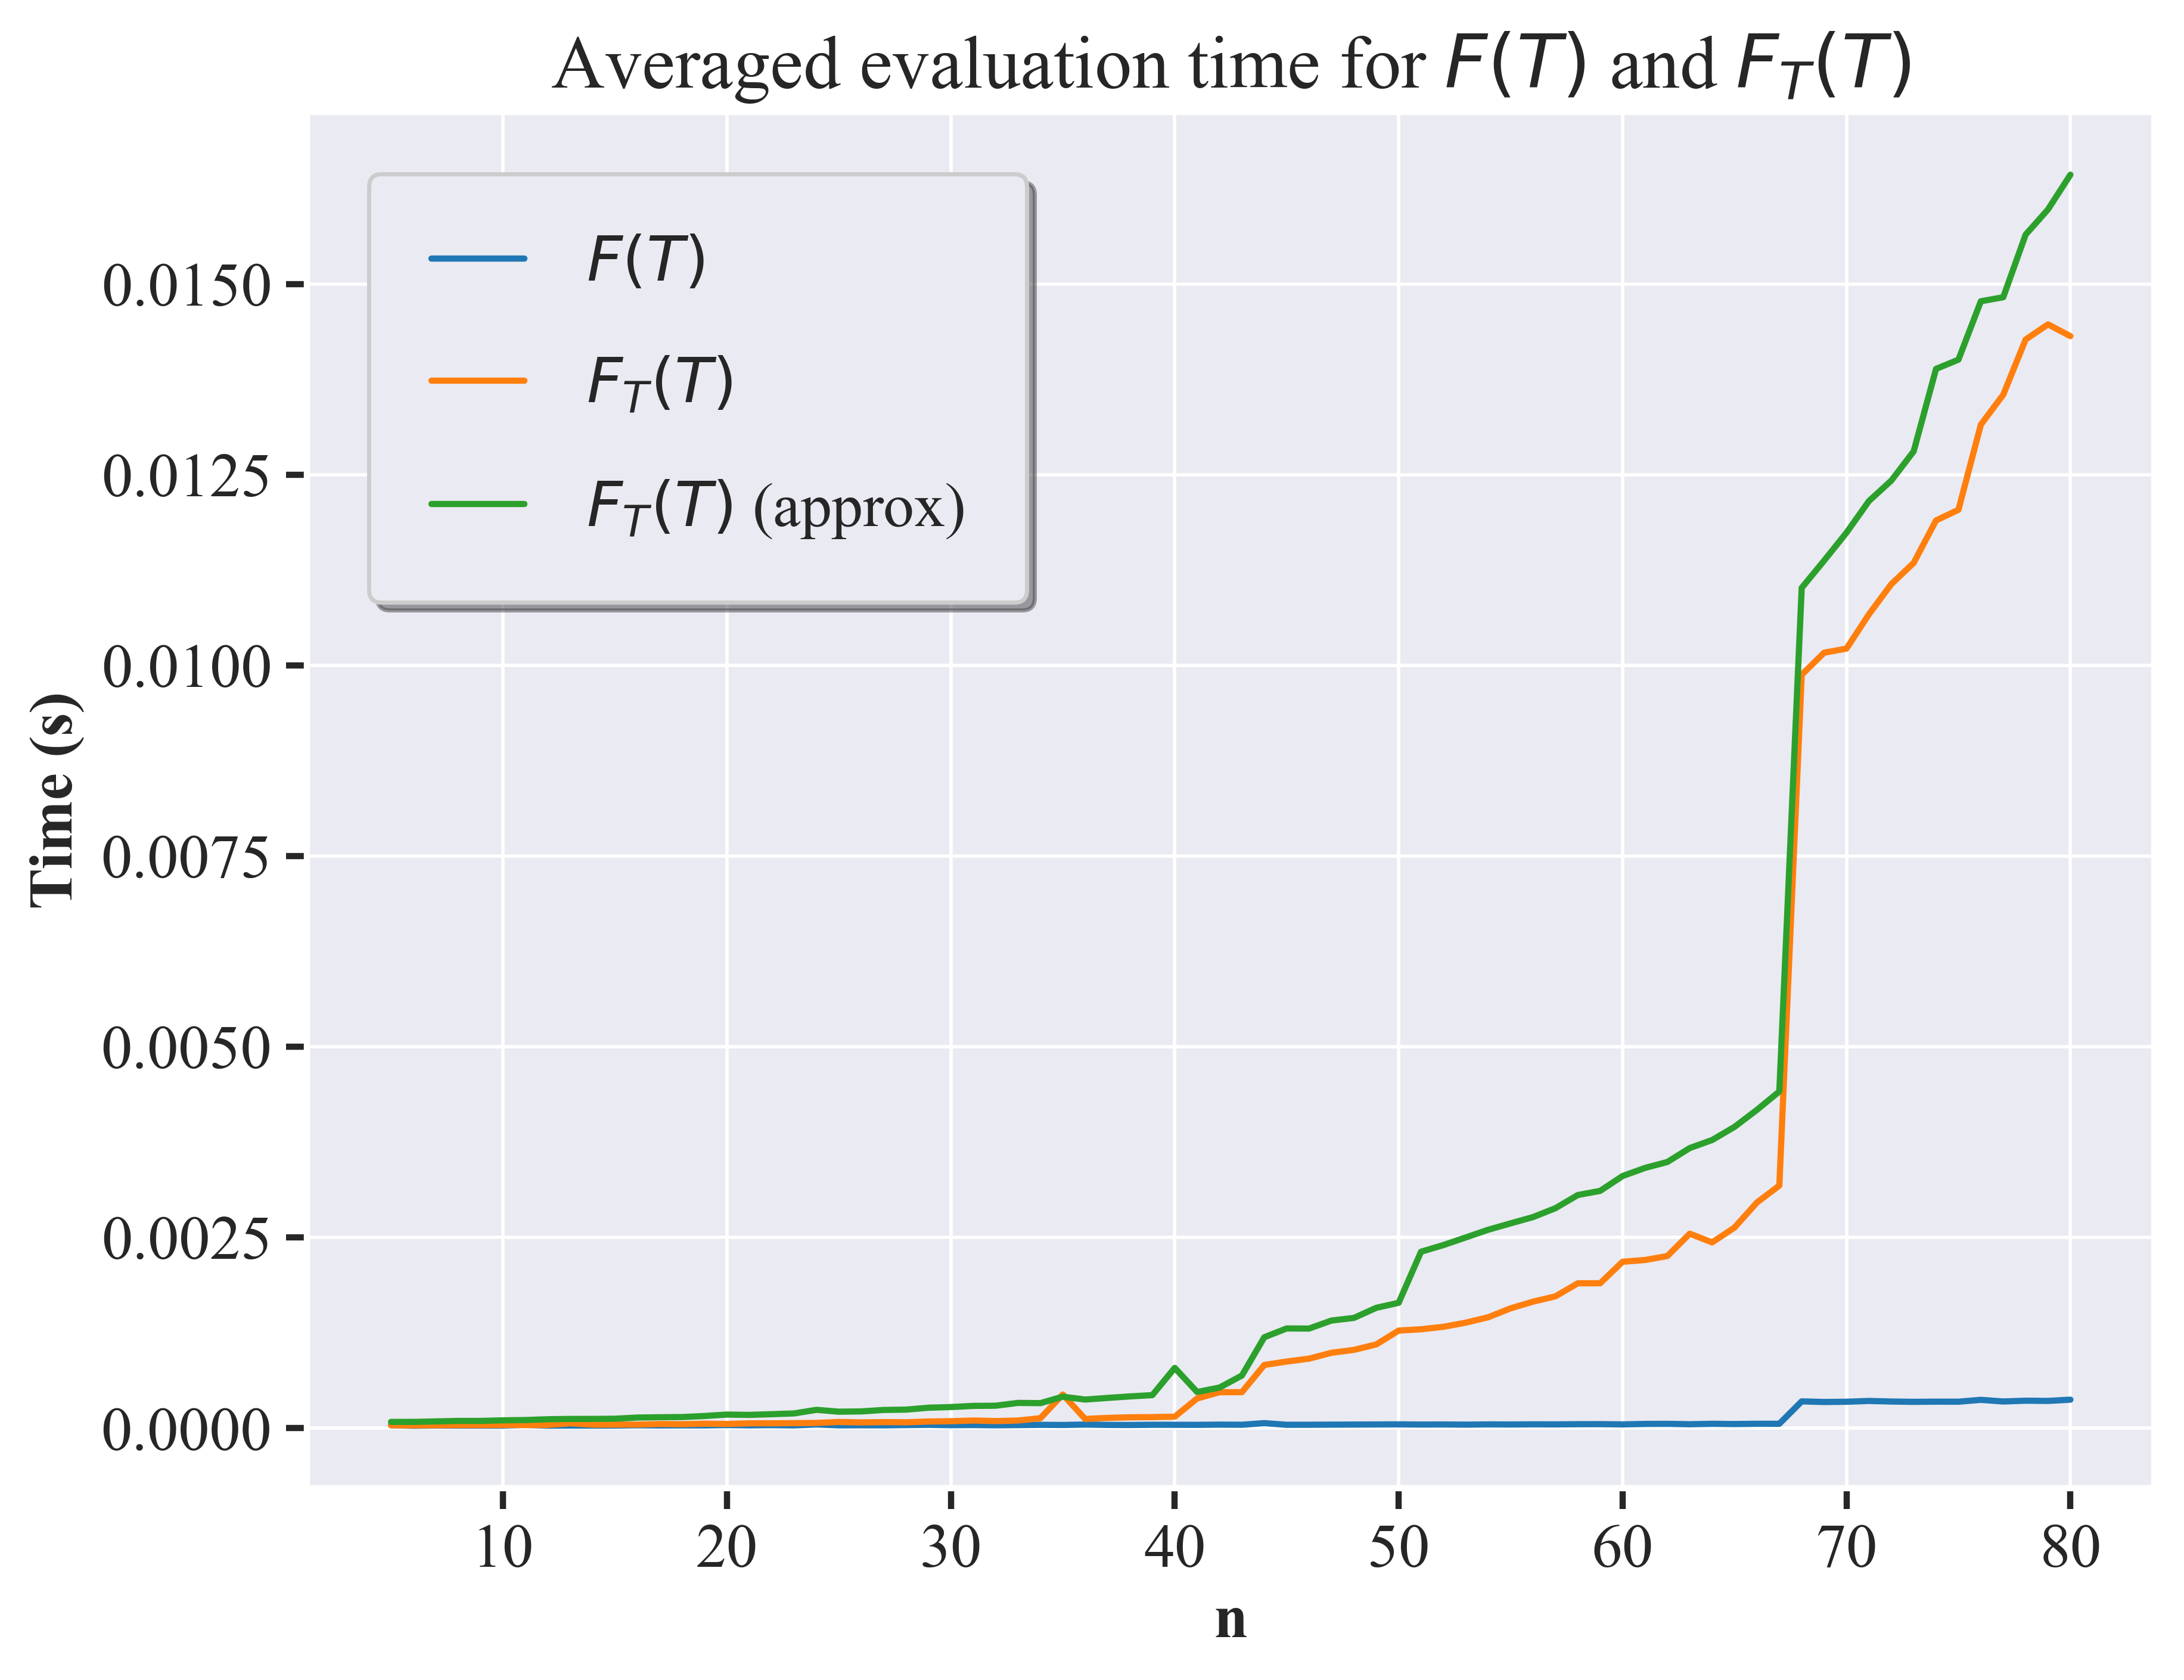
\includegraphics[width=\textwidth]{figures/function_evaluation_time_n=80.png}
        \caption{Computational time for one evaluation of the non-linear system and the jacobian using both the Galerkin and finite difference methods.}
        \label{fig:fd_vs_galerkin}
    \end{subfigure}
    \begin{subfigure}{0.45\textwidth}
        \centering
        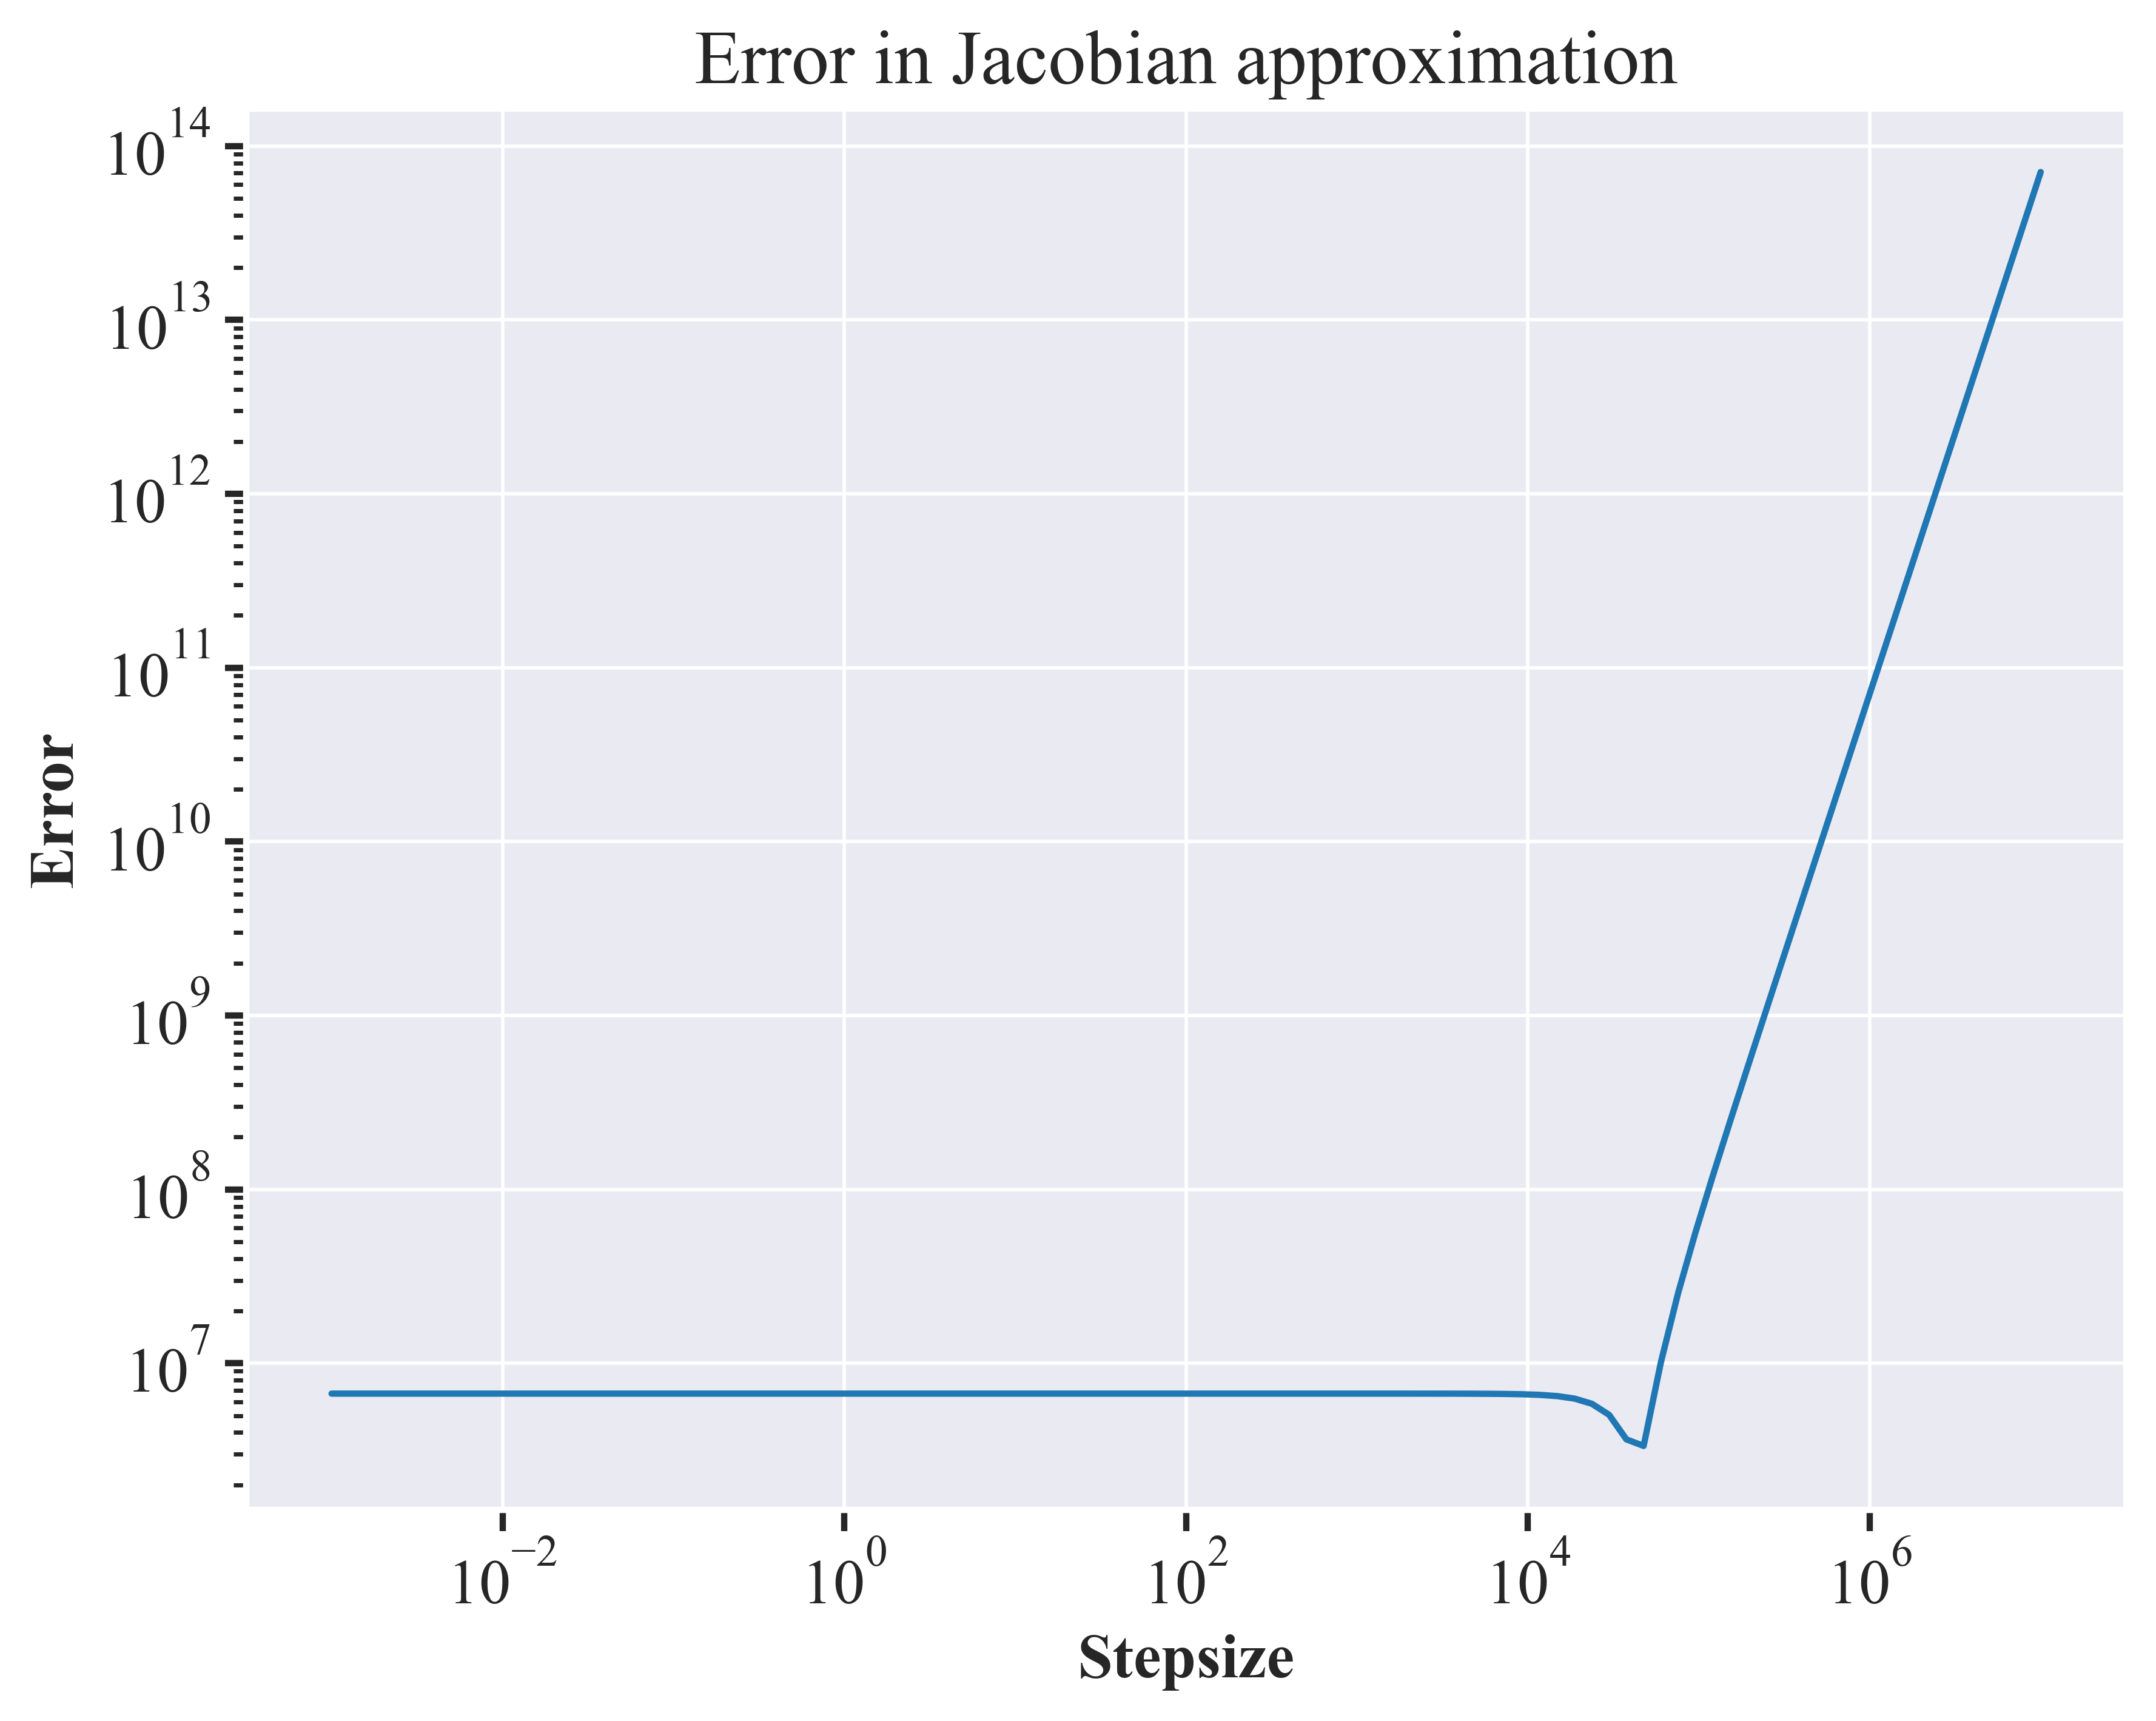
\includegraphics[width=\textwidth]{figures/jacobian_approximation_error.png}
        \caption{Comparison of the jacobian obtained using the Galerkin and finite difference methods for different values of $h$.}
        \label{fig:jac_comparison}
    \end{subfigure}
    \caption{Comparison of the Galerkin and finite difference methods.}
    \label{fig:fd_exact_comparison}
\end{figure}

As explained during the lectures, there exists an optimal value of $h$ for which the finite difference method is most accurate. 
From the \ref{fig:jac_comparison} we see that the finite difference method is most accurate for $h \approx 10^{-6}$. However, we also 
see from \ref{fig:fd_vs_galerkin} that the computational time for the finite difference method is comparable to the Galerkin method for problem
sizes with $n_p \leq 80$. This means that as far as this assignment is concerned, the Galerkin method is preferrable.

\subsection{Finding equilibria: Newton and Broyden}
Figure \ref{fig:equilibria} shows the equilibria found using the Newton and Broyden methods. 
\begin{figure}[H]
    \centering
    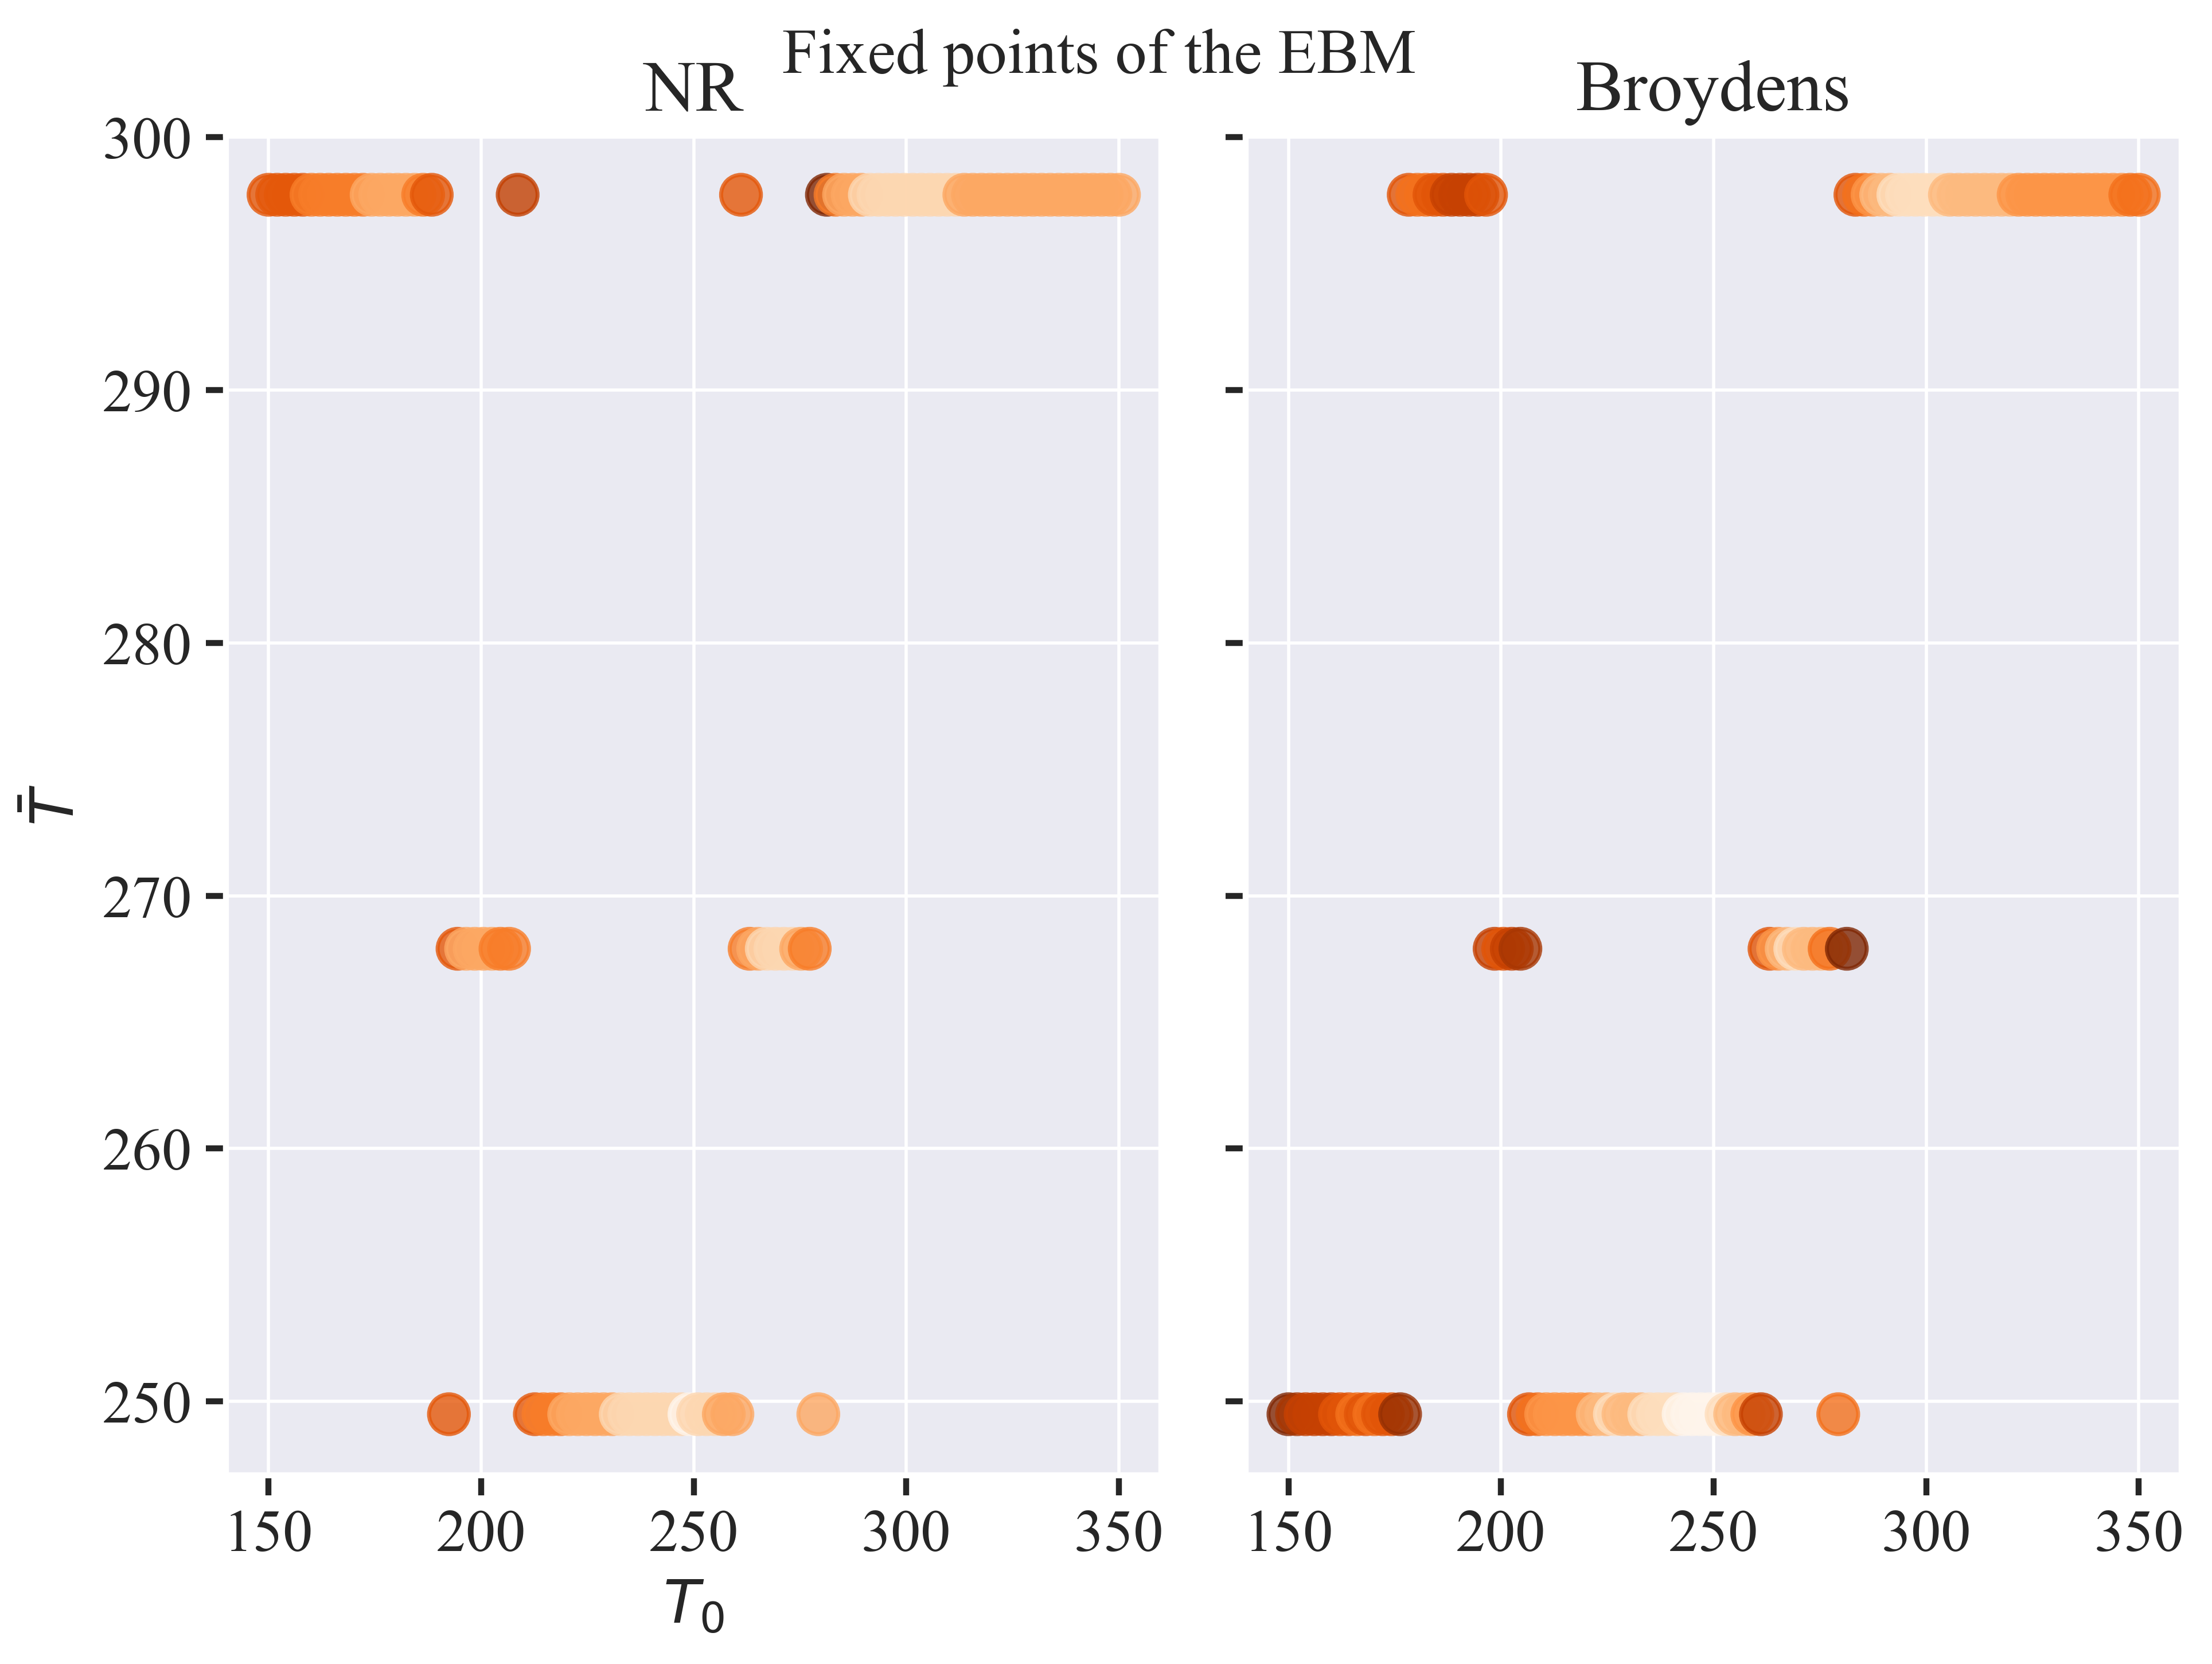
\includegraphics[width=0.7\textwidth]{figures/fixed_points.png}
    \caption{Equilibria found using the Newton and Broyden methods for a range of homogeneous initial temperatures $T_0$. 
    The color intensity indicates the amount of iterations required to converge.
    a high intensity indictes the method needed a low amount of iterations to converge.}
    \label{fig:equilibria}
\end{figure}
We notice that roughly speaking the equilibria found using the Newton and Broyden methods are the same. However, the Broyden method
seems to be less predictable in terms of to what root it converges. It is not directly clear how to compare domains of attraction 
for these two methods. However, we can see that the Newton method is more predictable in terms of the number of iterations required to converge and
what initial state ends up convering to what root. In other words, the Broyden method seems to be more sensitive to the initial state.
This might be due to the fact that the Broyden method's linear compated to Newton method's quadratic convergence rate causes it to 'skip' roots.

In terms of the state of our model Earth, we discover three distinct average temperatures $T_{eq} \approx 250 K$, $T_{eq} \approx 268 K$ and $T_{eq} \approx 298 K$.
The first corresponds to a frozen Earth, the second to a partially frozen Water world and the third to quite a cozy Blue Marble.

\subsection{Embedding}
    We can reduce the problem of finding the first equilibrium through the following embedding of the energy balance equation
    \begin{equation}
        f = \gamma R_D[T] + (1-\gamma)(R_A(T, x) + R_E(T)).
    \end{equation}
    Taking $\gamma = 0$ we obtain a transcendental equation for the equilibrium temperature, which we can easily solve using the Newton method.
    Once we have this solution we increment $\gamma$ and apply some continuation scheme using the methods for evaluating the non-linear system and
    its jacobian. This way we can find the other equilibria. We repeat this until we reach $\gamma = 1$, at which point we find an initial equilibrium.
    
\subsection{Bifurcation diagrams}
    The pseudo arclength continuation is implemented by first introducing the parametrisation $(T, \mu)\mapsto(T(s), \mu(s))$. This results in a extended 
    system of equations, which is the original system with an additional parametrisation equation.
    \begin{align*}
        \begin{cases}
            F(T(s), \mu(s)) = 0,\\
            p(T, \mu, s) = 0.
        \end{cases},
    \end{align*}
    where 
    \begin{align*}
        p(T, \mu, s) = 2\zeta(T - \bar{T})\frac{d T}{ds} + 2(1-\zeta)(\mu - \bar{\mu})\frac{d \mu}{ds} - \Delta s,
    \end{align*}
    where $(\bar{T}, \bar{\mu})$ denote the current equilibrium, $(T, \mu)$ the continued (as of yet uknown) solution, 
    $\zeta$ is a tune factor and $\Delta s$ is the arclength or step size

    The jacobian of this system is given by
    \begin{align*}
        \tilde{F}' = 
        \begin{bmatrix}
            \frac{\partial F}{\partial T} & \frac{\partial F}{\partial \mu}\\
            \frac{\partial p}{\partial T} & \frac{\partial p}{\partial \mu}
        \end{bmatrix},
    \end{align*}
    which after discretisation becomes
    \begin{align*}
        \textrm{D}\tilde{F} = 
        \begin{bmatrix}
            \frac{\partial \mathbf{F}}{\partial \mathbf{a}} & \frac{\partial \mathbf{F}}{\partial \mu}\\
            2\zeta\left(\frac{d \mathbf{T}}{ds}\right)^T & 2(1-\zeta)\frac{d \mu}{ds}
        \end{bmatrix}.
    \end{align*}
    The above system can be solved using the Newton method. The condition for convergence is such that the update
    \begin{align*}
        \begin{bmatrix}
            \Delta \mathbf{a}\\
            \Delta \mu
        \end{bmatrix} = -\left(\textrm{D}\tilde{F}\right)^{-1}\begin{bmatrix}
            \mathbf{F}\\
            p
        \end{bmatrix},
    \end{align*}
    must be smaller than some tolerance $\epsilon = 10^{-5}$.
    	
    Figure \ref{fig:bifurcation} shows the bifurcation diagram for the Earth model. This figure was made by rerunning
    the continuation scheme for different initial temperatures $T_0$ and plotting the equilibria found. 
    \begin{figure}[H]
        \centering
        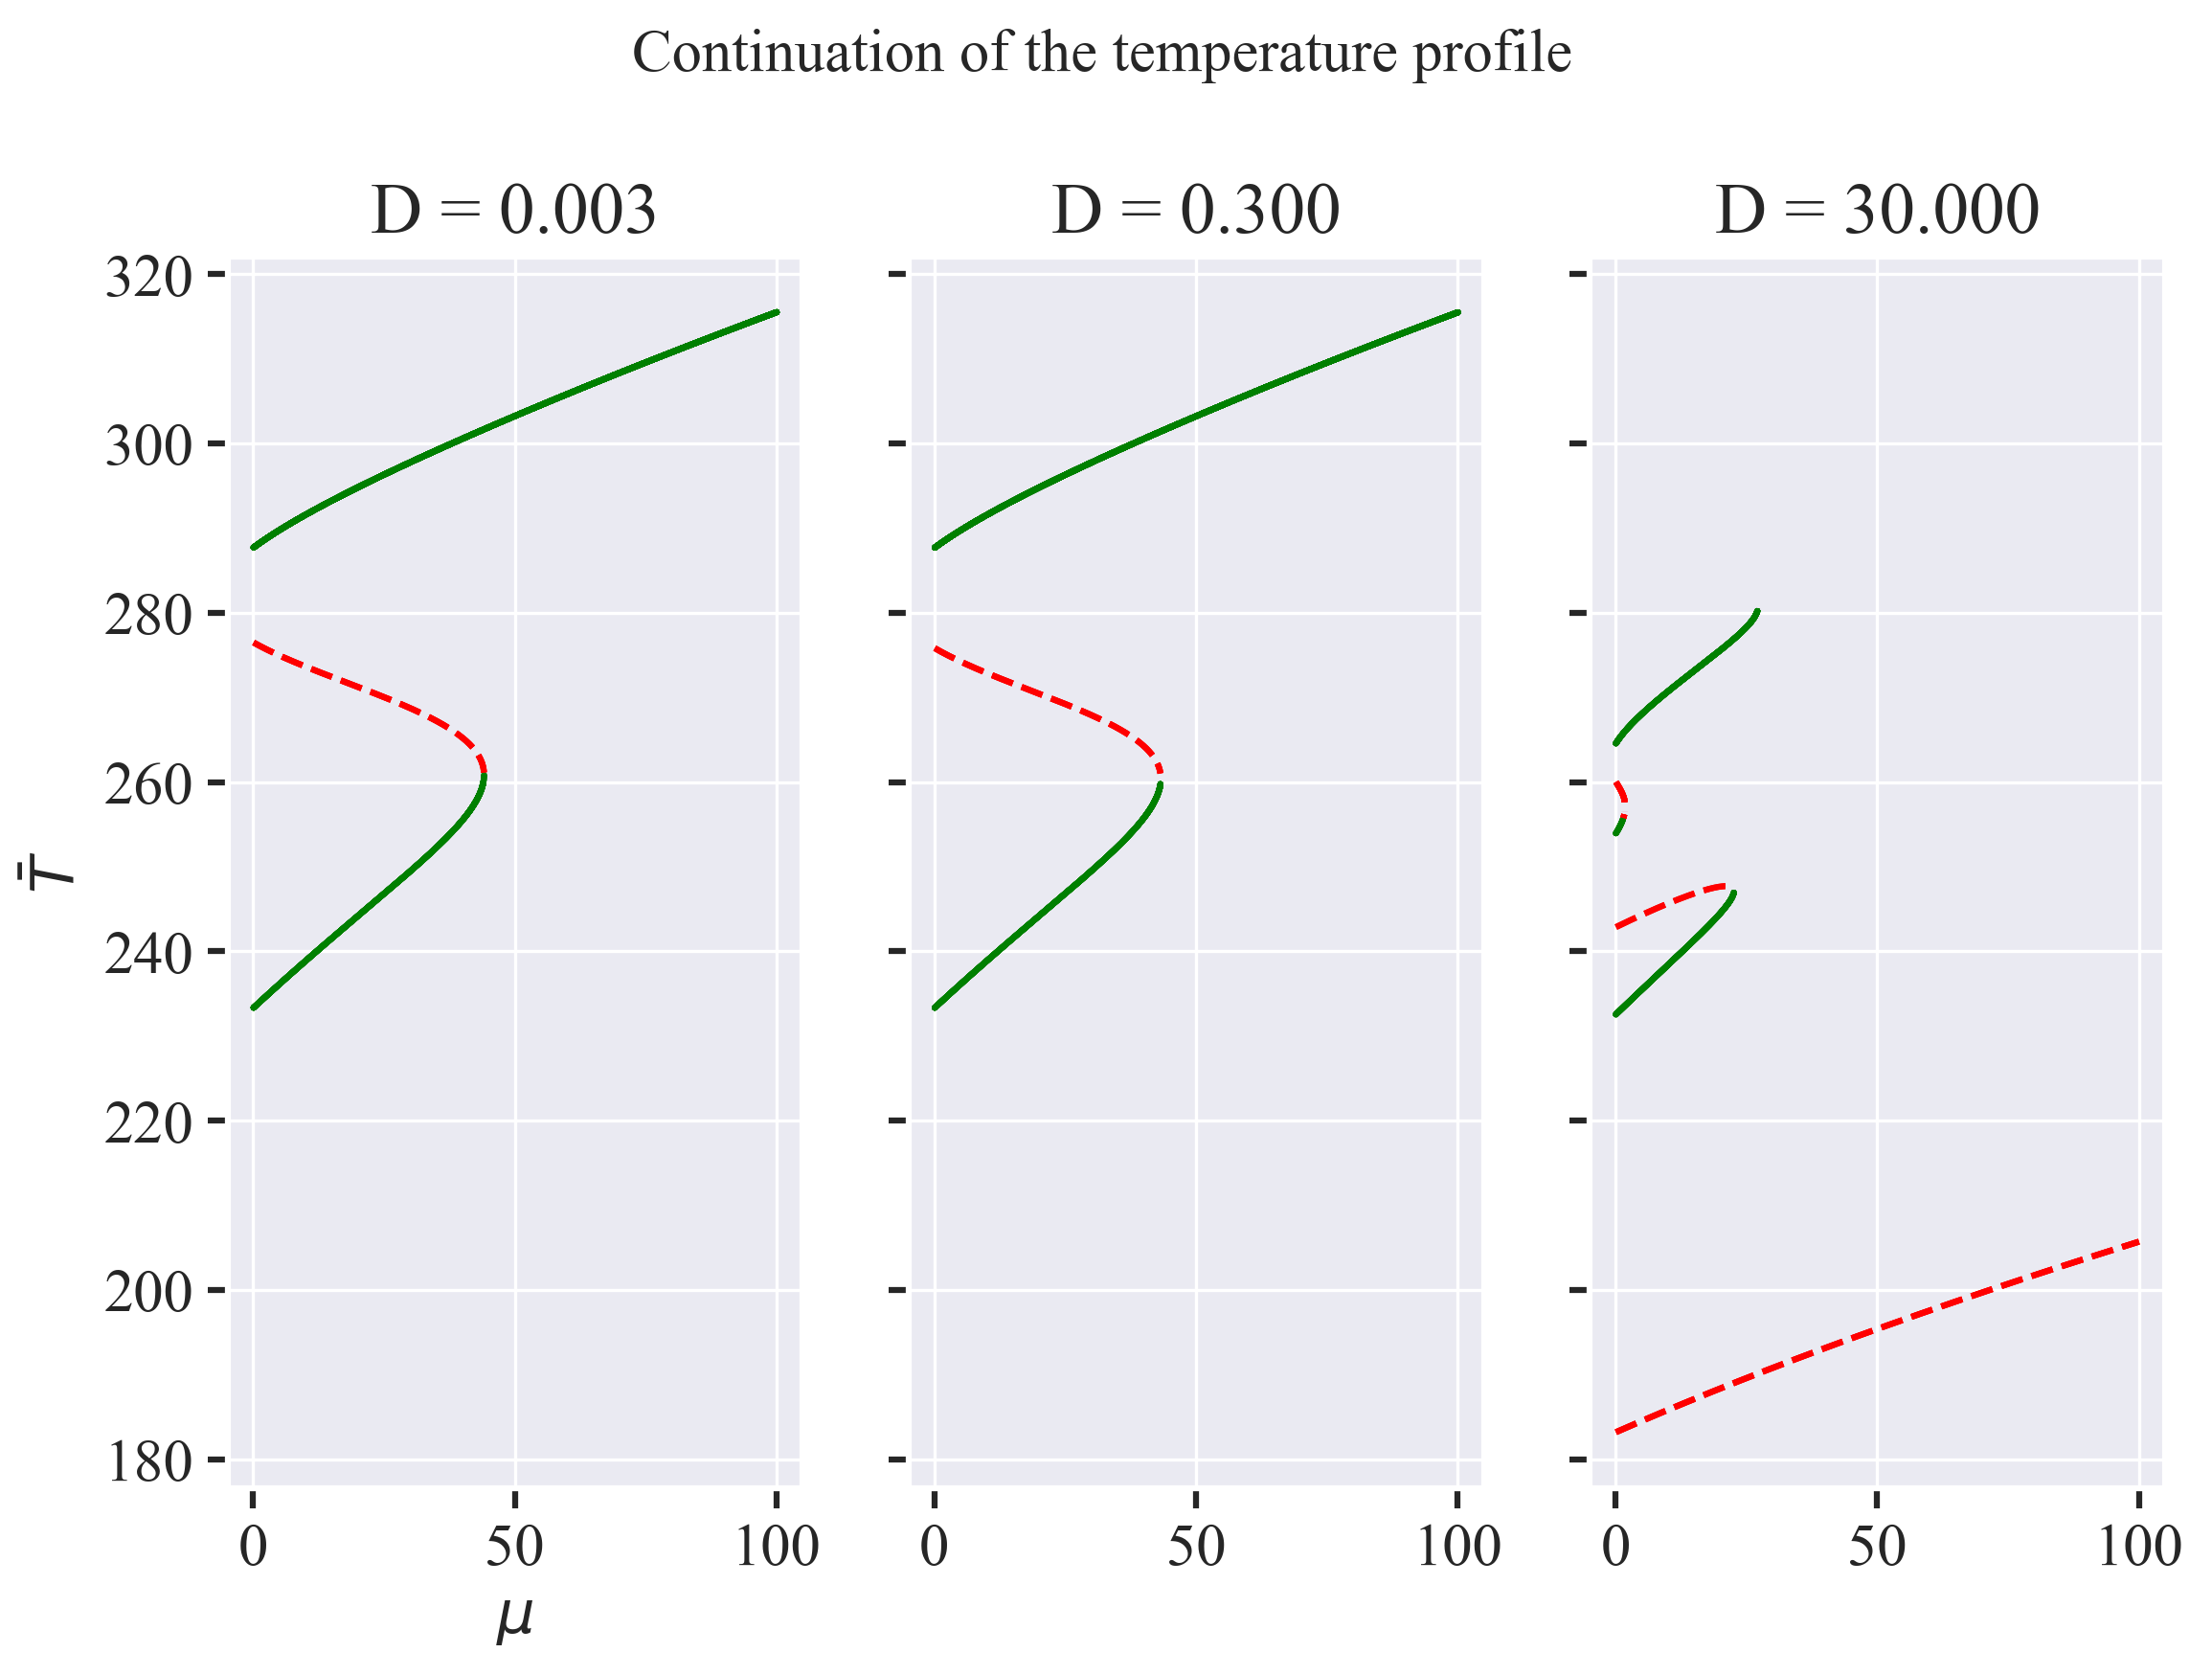
\includegraphics[width=0.8\textwidth]{figures/ebm_continuation.png}
        \caption{Bifurcation diagram for the Earth model. Green solid lines indicates a stable branch
        while red, dashed lines indicate an unstable branch.}
        \label{fig:bifurcation}
    \end{figure}

    A typical temperature profile is given in Figure \ref{fig:temperature_profile}. We see that the temperature profile is symmetric around the equator, which is expected.
    \begin{figure}[H]
        \centering
        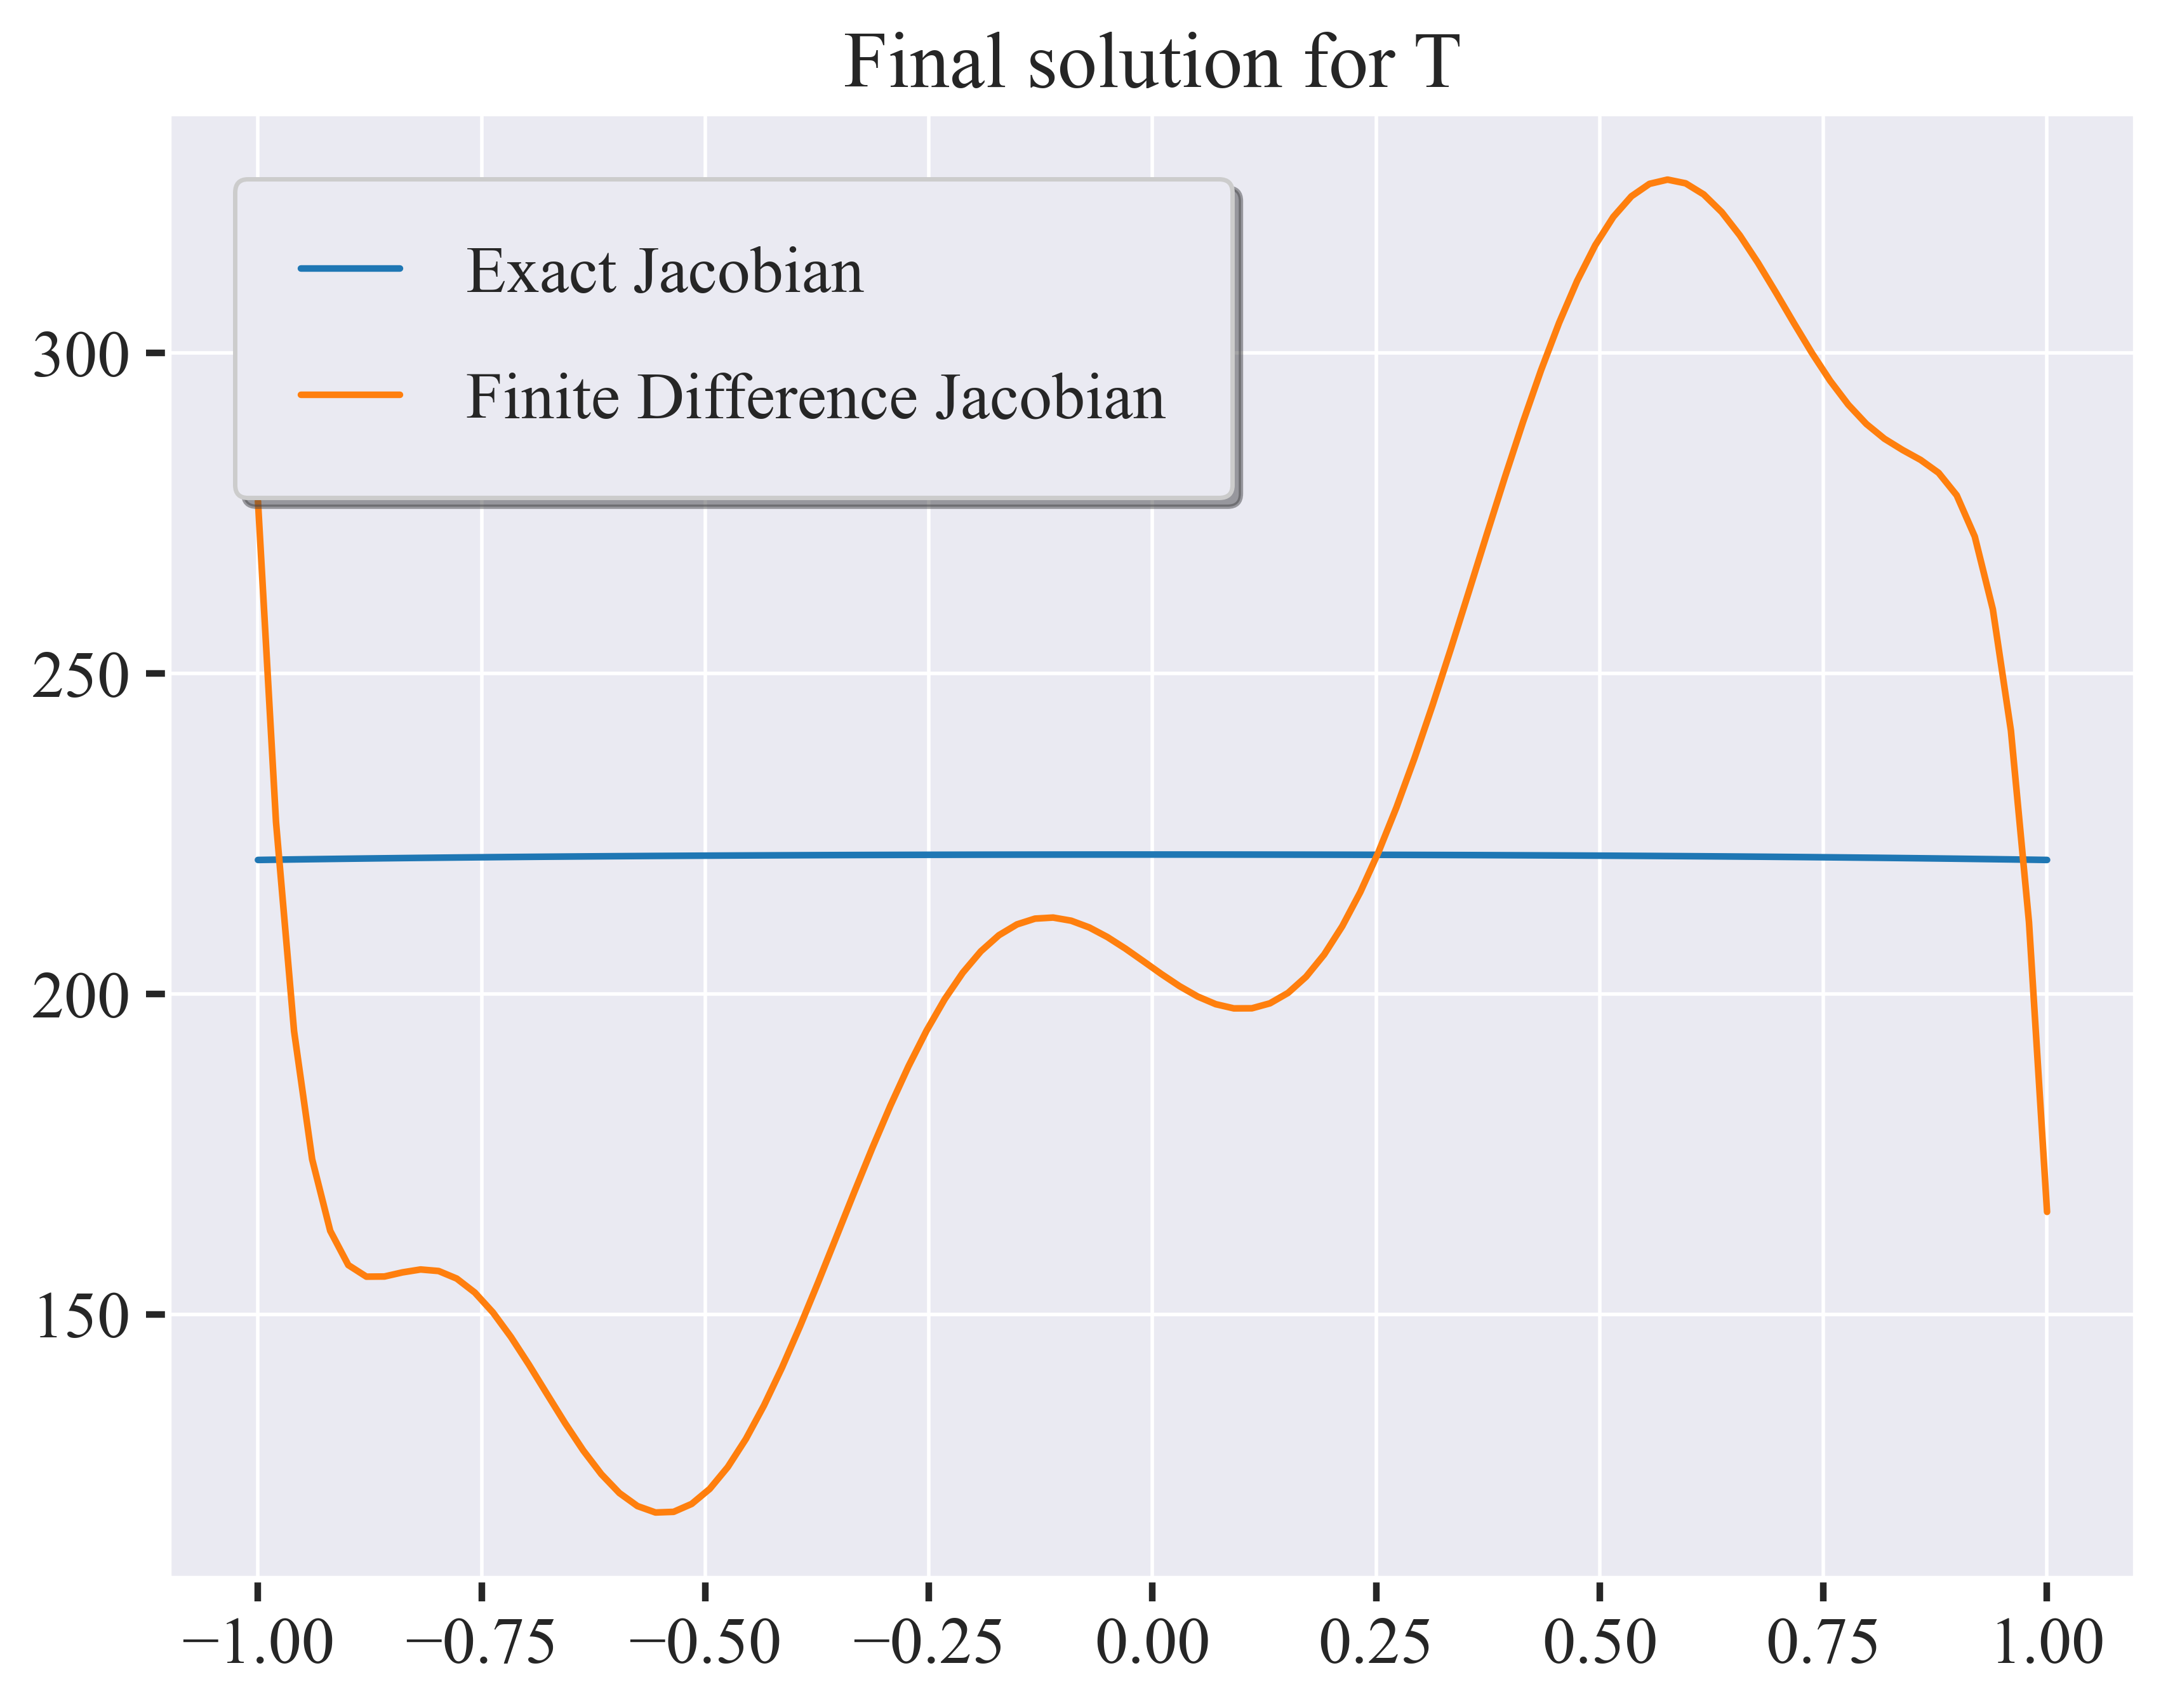
\includegraphics[width=0.7\textwidth]{figures/equilibrium_T.png}
        \caption{Typical temperature profile for the Earth model.}
        \label{fig:temperature_profile}
    \end{figure}

    We see from Figure \ref{fig:bifurcation} that we need a small step size to accurately resolve all the branches in the bifurcation diagram ($\Delta s \leq 0.1$).
    Additionally, we should place emphasis on tracking small changes in the parameter ($\zeta \leq 0.001$).

    In figure \ref{fig:bifurcation} we solely identify fold (subtle) and jump (critical) bifurcations.
    
    Next to this we recover the three equilibria found above. For small values of the diffusion constant $D=0.003, 0.3$ we find that for $\mu\gtrapprox50$ there is only 
    one stable branch. In case of the partially frozen Earth, we see that increasing $\mu$ at first has the effect of lowering the temperature.
    However, at some point it appears the greenhouse effect becomes strong enough to counteract the cooling effect of the ice the solution suddenly jumps to the
    aforementioned stable branch.
    
    This behaviour is radically different however for $D=30$. We suddenly see many more branches appearing. This is due to the fact that the heat dispersion is so strong
    that the temperature gradient is much steeper. This results in initially completely ice covered earths to become unstable.


\subsection{Conclusion}
    We have found the equilibria of the Earth model and studied the bifurcation diagram. We have seen that for default parameter values the Earth model has three distinct equilibria, 
    corresponding to a frozen, a partially frozen and a warm Earth. We have also seen that the bifurcation diagram is sensitive to the 
    diffusion constant $D$. For small values of $D$ we see that the bifurcation diagram is relatively simple, with only fold and jump bifurcations. However, for 
    large values of $D$ the bifurcation diagram becomes much more complex, with many more branches appearing. This is due to the fact that the heat dispersion is so 
    strong that the temperature gradient is much steeper. This results in initially completely ice covered earths to become unstable.